\begin{frame}
    \frametitle{La plateforme IRIS}
    \framesubtitle{Imagerie, Robotique et Innovation en Santé}
    \begin{block}{Le rôle}
    La plateforme IRIS  offre les moyens et un support à la recherche en Imagerie, en Robotique et l'Innovation pour la Santé
    \end{block}
    \begin{block}{Nos missions}
        Fournir une expertise et un environnement à la fois matériel et logiciel permettant :
        \begin{itemize}
            \item le développement et l'optimisation de protocole d'imagerie biomédicale (IRM, Ultrason, imagerie optique, etc.) ;
            \item l'élaboration et l'évaluation de dispositifs pour l'imagerie médicale et biomédicale multimodale ;
            \item le développement d'assistant robotique pour le GMCAO (hardware et software) ; 
            \item l'analyse et le traitement des données ;
            \item la réalisation d'études cliniques et pré-cliniques ;
            \item essais biomécaniques; 
        \end{itemize}
    \end{block}
\end{frame}
%=====================================================================================================================================
\begin{frame}
    \frametitle{La plateforme IRIS}
    \framesubtitle{Un emplacement unique}
    Située dans l'enceinte de l'hôpital Civil de Strasbourg, répartie sur 3 sites avec près de 1500 m$^2$ de surface :
    \begin{itemize}
        \item Nouvel Hôpital Civil (NHC), IRM Interventionnelle dans le service d'imagerie interventionnelle du Pr. Gangi ;
        \item Institut Hospitalo-Universitaire (IHU), plateau technique robotique et mécatronique ;
        \item Institut de Physique Biologique (IPB), imagerie homme et pré-clinique, biomécanique et informatique.
    \end{itemize}
    \begin{figure}[!h]
        \centering
            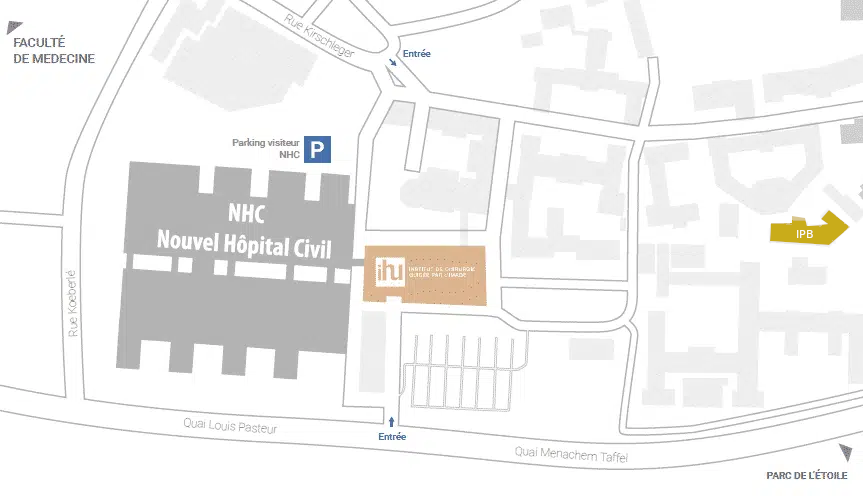
\includegraphics[height=4cm]{img/plan-acces.png.png}
    \end{figure}
\end{frame}
%=====================================================================================================================================
\begin{frame}
    \frametitle{La plateforme IRIS}
    \framesubtitle{Réseaux et labelisation}
    \begin{itemize}
        \item IRIS est impliquée dans plusieurs réseaux régionaux et nationaux
    \end{itemize}
    \begin{columns}
        \column{0.3\textwidth}    
        \begin{figure}[!h]
            \centering
                
\includegraphics[height=0.7cm]{logos/reseaux_labelisation/nyg_nouleur-2.png}
                \caption*{FHU Neurogeneti$\Phi$cs, Strasbourg}
        \end{figure}  
        \column{0.3\textwidth}    
        \begin{figure}[!h]
            \centering
                
\includegraphics[height=0.7cm]{logos/reseaux_labelisation/logo_FMTS.jpg}
                \caption*{Fédération de Médecine Translationnelle de Strasbourg}
        \end{figure}  
        \column{0.3\textwidth}    
        \begin{figure}[!h]
            \centering
                
\includegraphics[height=0.7cm]{logos/reseaux_labelisation/neuropole_photo_large.jpg}
                \caption*{Neuropole - Pôle des Neurosciences de Strasbourg}
        \end{figure}              
    \end{columns}
    % ROBOTEX 2.0
    \begin{columns}
        \column{0.3\textwidth}
            \begin{figure}[!h]
                \centering
                    
\includegraphics[height=0.7cm]{logos/reseaux_labelisation/ROBOTEX2.0-V1.png}
            \end{figure} 
        \column{0.7\textwidth}
            ROBOTEX2.0 réseau des plateformes nationales  de robotique.
    \end{columns}
    % FLI
    \begin{columns}
        \column{0.3\textwidth}
            \begin{figure}[!h]
                \centering
                
\includegraphics[height=0.7cm]{logos/reseaux_labelisation/FLI_Logotype_Coul-5cm.jpg}
            \end{figure} 
        \column{0.7\textwidth}
            FLI, France Life Imaging.
    \end{columns}
    % IBISA
    \begin{columns}
        \column{0.3\textwidth}
            \begin{figure}[!h]
                \centering
                
\includegraphics[height=0.7cm]{logos/reseaux_labelisation/IBISA.png}
            \end{figure} 
        \column{0.7\textwidth}
            IBISA, Infrastructure en Biologie, Santé et Agronomie
    \end{columns}
    % CARNOT TSN
    \begin{columns}
        \column{0.3\textwidth}
            \begin{figure}[!h]
                \centering
                
\includegraphics[height=0.7cm]{logos/reseaux_labelisation/logo Carnot TSN.jpg}
            \end{figure} 
        \column{0.7\textwidth}
            CARNOT, Télécom \& Société Numérique
    \end{columns}
\end{frame}

%=====================================================================================================================================
\begin{frame}
    \frametitle{La plateforme IRIS}
    \framesubtitle{6 pôles d'expertises}
    \begin{itemize}
        \item Neuro-Imagerie Homme :
        \item Imagerie Pré-Clinique :
        \item Imagerie Interventionnelle :
        \item Biomécanique :
        \item Robotique :
        \item Informatique et Traitement d'Images :
    \end{itemize}
\end{frame}